% !TEX root =path to root.tex
\documentclass[a4paper,12pt]{report} 

\usepackage[utf8]{inputenc}          
\usepackage[italian]{babel}
\usepackage{amsmath, amssymb}         
\usepackage{graphicx}                 
\usepackage{hyperref}                 
\usepackage{geometry}                 

\geometry{left=3cm, right=3cm, top=3cm, bottom=3cm}

\begin{document}

\title{Studio sul Gioco del Domino}
\author{Alex Lorenzato}

\maketitle
\tableofcontents 

% \footnote{Fonte: Wikipedia, \emph{Teoria dei giochi}, \url{https://it.wikipedia.org/wiki/Teoria_dei_giochi} (accesso il 12 Dicembre 2024).}

%%%%%%%%%%%%%%%%%%%% INTRODUZIONE %%%%%%%%%%%%%%%%%%%%
\chapter{Introduzione}

\section{Il Domino}

Il domino è un antico gioco da tavolo le cui origini risalgono alla Cina imperiale. 
Le tessere di gioco sono rettangolari e suddivise in due metà: su ciascuna metà è presente un valore numerico che va da 0 a 6, rappresentato tipicamente con dei pallini, o "pip", che indicano il punteggio della tessera. 
Le tessere formano una combinazione unica di numeri, con 28 tessere totali in un set "double-six" (rappresentato in figura 1.1), ovvero la cui tessera di maggior valore è quella in cui appaiono due 6.

L'obiettivo generale del gioco, sebbene esistano diverse varianti, è di liberarsi di quante più tessere possibili dalla propria mano prima della fine della partita. 

Il gioco procede a turni in senso orario: ogni giocatore, nel suo turno, ha la possibilità di aggiungere una tessera dalla propria mano all'inizio o alla fine della sequenza di tessere presenti sul tavolo, rispettando la condizione che il valore su una delle estremità della tessera coincida con il valore della tessera a cui si collega. 

Nella variante classica, la partita inizia con il giocatore che possiede la tessera doppia con il valore più alto, di conseguenza il doppio-6 è la tessera che garantisce di partire per primi. Questa versione è particolarmente popolare nella modalità a 2 giocatori, ma può essere giocata anche da un massimo di 4 o 6 giocatori, con regole e adattamenti per gestire il numero di tessere e i turni.

\begin{figure}[h!]
    \centering
    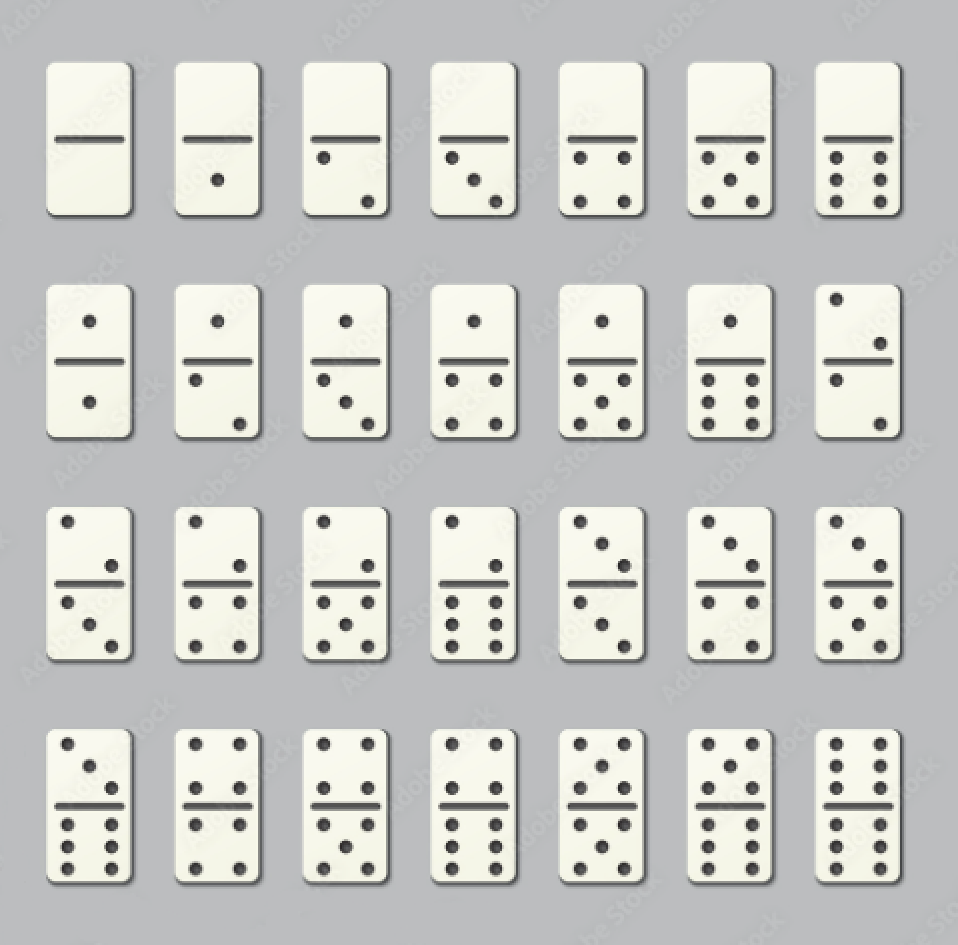
\includegraphics[width=1\textwidth]{imgs/domino_set.png} 
    \caption{Set base di tessere del domino}
    \label{fig:domino_set}
\end{figure}

\begin{figure}[h!]
    \centering
    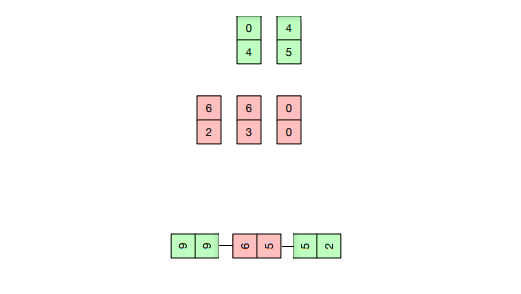
\includegraphics[width=1\textwidth]{imgs/domino_table.png} 
    \caption{Esempio di partita in corso}
    \label{fig:game_example}
\end{figure}

\vspace{0.5cm}

Nella figura 1.2 è rappresentato un piccolo esempio di partita in corso:

\begin{itemize}
    \item Il giocatore 1 è il verde, che ha iniziato giocando la tessera \(6|6\)
    \item Il giocatore 2, rosso, ha scelto di giocare la tessera \(6|5\), le alternative erano la \(6|2\) e \(6|3\)
    \item Il giocatore 1 risponde scegliendo la tessera \(5|2\), l'alternativa era la \(4|5\)
        \item Ora è il turno del giocatore 2 che ha 3 mosse dispnibili: la \(6|2\) può andare sia in testa che in coda, oppure la \(6|3\)
\end{itemize}


% STORIA DEL DOMINO %
\section{Storia del Domino}

Il domino con tessere nacque in Cina intorno al XII secolo e si ritiene che sia stato sviluppato da uno statista nel 1120, come dono per l'imperatore Hui Tsung. 

Inizialmente, il domino aveva anche un ruolo come strumento di divinazione intorno al XIII secolo, diventando poi un gioco da tavolo vero e proprio.

Nel corso del tempo, il gioco del domino si diffuse dal continente asiatico all'Europa, probabilmente grazie agli scambi culturali mediati dal mondo arabo. Giunto in Italia, il gioco si diffuse rapidamente in Francia e successivamente in tutta Europa. Il termine "domino" deriva dal latino \textit{dominus}, che significa "padrone", e sembra essere legato al senso di controllo e strategia che il gioco richiede.\footnote{Fonte: Wikipedia, "Domino", https://it.wikipedia.org/wiki/Domino (accesso il 25 ottobre 2024).}


% VARIANTE BLOCK %
\section{Variante "Block"}

La variante "Block" è la versione del domino utilizzata come oggetto di studio in questa tesi, nonché la variante più diffusa e popolare.

Questa versione utilizza un set di tessere "double-six", ovvero tessere con valori che vanno da 0 a 6 su ciascuna metà. 

Ogni giocatore pesca sette tessere all'inizio del gioco, e le rimanenti 14 tessere vengono scartate e non utilizzate per tutta la durata della partita. 

La partita termina in due casi:

\begin{enumerate}
    \item Quando un giocatore riesce a liberarsi di tutte le tessere in mano, vincendo automaticamente.
    \item Quando la partita è "bloccata", ossia nessuno dei due giocatori può posizionare una tessera valida.
\end{enumerate}

In caso di "blocco", vince il giocatore con il minor punteggio totale in mano, dove il punteggio è calcolato come la sommatoria dei valori presenti sulle tessere rimanenti in mano ai giocatori. 

Se un giocatore riesce a esaurire tutte le sue tessere, è dichiarato automaticamente vincitore.

Un esempio: il giocatore 1 a fine partita ha in mano le tessere \(0|4, 6|5\) e il giocatore 2 la tessera \(3|4\) allora il giocatore 1 accumula 15 punti mentre il giocatore 2 solo 7 punti; lo scopo quindi è avere un punteggio il più basso possibile.


% ALTRE VARIANTI %
\section{Altre varianti}

Assieme alla variante "Block", esiste la variante "Draw", che differisce per l'uso delle tessere non distribuite ai giocatori. 

Mentre nella "Block" le tessere avanzate vengono rimosse definitivamente dalla partita, nella variante "Draw" i giocatori possono pescare tessere aggiuntive quando non riescono a fare una mossa valida. 

Le modalità di pesca variano: in alcune versioni il giocatore è obbligato a pescare fino a trovare una tessera giocabile, mentre in altre può pescare solo una tessera per turno.

Queste varianti danno origine a una vasta gamma di regole aggiuntive e variazioni del gioco. 

Esistono inoltre numerose versioni del domino fan-made e competitive, ognuna con modifiche più o meno significative alle regole delle varianti "Block" e "Draw". 

Per esempio, oltre all’obiettivo tradizionale di esaurire la propria mano, alcune modalità premiano configurazioni particolari di tessere sul tavolo, rendendo il gioco ancora più strategico e vario.



%%%%%%%%%%%%%%%%%%%% TEORIA DEI GIOCHI %%%%%%%%%%%%%%%%%%%%
\chapter{Teoria dei giochi}

La teoria dei giochi è una disciplina che studia modelli matematici di interazione strategica tra agenti razionali.
La teoria dei giochi ha applicazioni in vari campi delle scienze sociali, così come nella logica, nella teoria dei sistemi e nell'informatica. 
Sebbene originariamente si sia focalizzata sui giochi a somma zero, in cui i guadagni o le perdite di ogni partecipante sono perfettamente bilanciati da quelli degli altri, la teoria dei giochi contemporanea si applica ad una vasta gamma di relazioni comportamentali 
e indica ormai genericamente la scienza delle decisioni logiche negli esseri umani, negli animali e nei calcolatori.\footnote{Fonte: Wikipedia, \emph{Teoria dei giochi}, \url{https://it.wikipedia.org/wiki/Teoria_dei_giochi} (accesso il 12 Dicembre 2024).}
Lo studio del gioco del domino ricade pienamente nella disciplina della teoria dei giochi, nelle prossime sezioni ne verranno approfonditi alcuni aspetti tecnici.


\section{L'albero di gioco}

Un albero di gioco è una struttura utilizzata per rappresentare tutte le possibili sequenze di mosse in un gioco a turni, in questo caso il domino, partendo da una situazione iniziale fino a tutte le configurazioni finali possibili, dette "foglie" dell'albero. 

Ogni possibile situazione di gioco è rappresentata da un "nodo" dell'albero e ciascun "ramo" rappresenta una possibile mossa effettuata dal giocatore corrente.

Il nodo radice rappresenta lo stato iniziale, con le mani iniziali dei giocatori e il turno del primo giocatore. 

Ogni nodo discendente rappresenta uno stato raggiungibile in base alla tessera che un giocatore gioca.

L’albero di gioco ha lo scopo di esplorare tutte le mosse possibili per individuare le mosse ottimali, in modo da massimizzare la probabilità di vittoria. 

Accade molto facilmente che un albero di gioco si allarghi moltissimo, questo comporta un peso computazionale maggiore, ed è per questo che si possono adottare delle ottimizzazioni algoritmiche per ridurne la complessità e di conseguenza le tempistiche di calcolo.

\begin{figure}[h!]
    \centering
    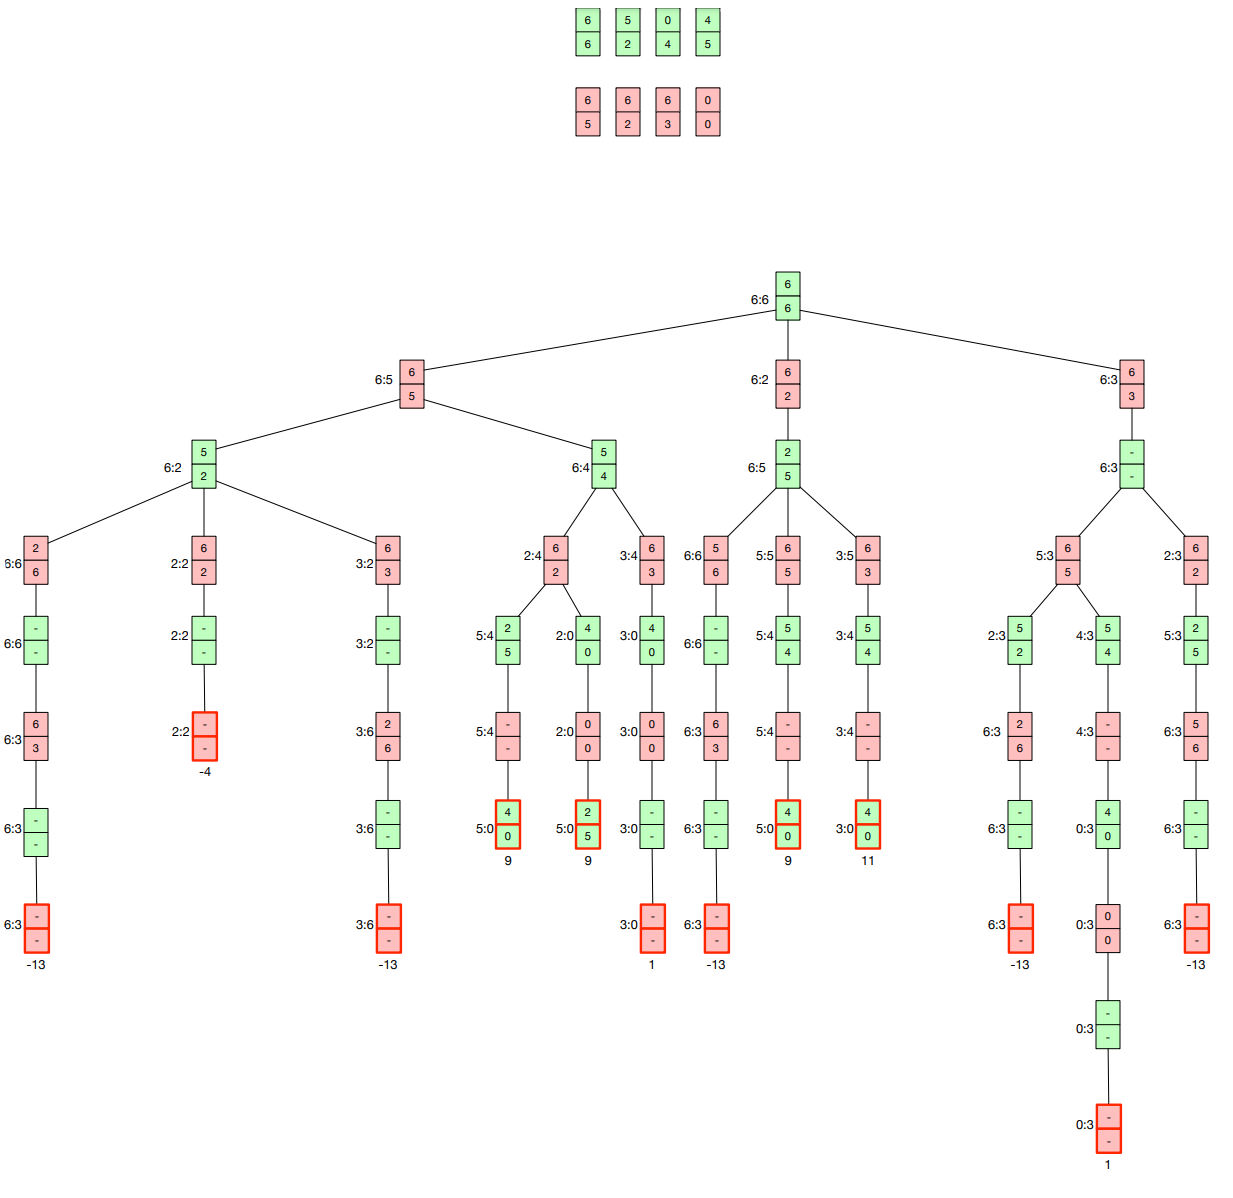
\includegraphics[width=1\textwidth]{imgs/gametree.png} 
    \caption{Esempio di albero di gioco}
    \label{fig:etichetta}
\end{figure}

In figura 1.3 si può vedere un esempio di albero da gioco, gli elementi sono i seguenti:

\begin{enumerate}
    \item i due set da 4 tessere rappresentati in cima sono le mani iniziali dei due giocatori
    \item il nodo radice, ovvero il \(6|6\) verde in cima all'albero, è la prima mossa giocata; il verde quindi è il giocatore 1 (iniziale)
    \item i 3 nodi immediatamente sotto sono le possibili mosse che può fare l'avversario
    \item i numeri rappresentati all'immediata sinistra di ogni tessera dell'albero sono il valore della testa e della coda nel tavolo facendo quella mossa
    \item le foglie sono le tessere dove l'albero si interrompe e ciascuna rappresenta un fine partita differente
    \item il numero sotto alle foglie rappresenta il punteggio di fine partita: positivo se vince il primo giocatore e viceversa  
\end{enumerate}

Il valore delle foglie è calcolato facendo la differenza tra i punti del giocatore 1 e quelli del giocatore 2, usando l'esempio del ramo più a sinistra:

\begin{itemize}
    \item il giocatore 1 (verde) rimane con le tessere \( 0|4, 4|5\) in mano, totalizzando 13 punti
    \item il giocatore 2 (rosso) rimane con la tessera \(0|0\) in mano, totalizzando 0 punti
    \item il giocatore 1 perde, il punteggio della foglia è banalmente dato dalla differenza \(13 - 0\)
\end{itemize}


% MINIMAX %
\section{Minimax}

Il principio del minimax, nella teoria dei giochi, consiste nel massimizzare il proprio punteggio minimizzando nel contempo quello dell'avversario.

Questo approccio presuppone che entrambi i giocatori siano perfettamente razionali, ossia giochino sempre la mossa migliore possibile a loro disposizione.
In un contesto reale questo è difficile che accada proprio per la complessità di calcolo derivante dallo studiare la mossa perfetta.

Nei giochi a turni, il principio del minimax assume la forma di algoritmo minimax: un algoritmo ricorsivo per la ricerca della mossa migliore in una determinata situazione. 

L'algoritmo minimax è costituito da una funzione di valutazione posizionale che misura la bontà di una posizione (o stato del gioco) e indica quanto è desiderabile per il dato giocatore raggiungere quella posizione.

Il giocatore fa poi la mossa che minimizza il valore della migliore posizione raggiungibile dall'altro giocatore. \footnote{Fonte: Wikipedia, \emph{Minimax}, \url{https://it.wikipedia.org/wiki/Minimax} (accesso il 12 Dicembre 2024).}

Minimax solitamente è rappresentato da una struttura ad albero il cui nodo radice è la situazione iniziale, le diramazioni portano ai nodi successivi che rappresentano le possibili mosse e di conseguenza le situazioni che ne derivano.

Reiterando questo processo si arriva fino alle foglie, dove l'albero smette di crescere in quanto il fine partita è stato raggiunto.

Una volta calcolate tutte le foglie, che ricordo rappresentano situazioni di fine partita, il Minimax valuta il punteggio di ciascuna di esse e "risale" l'albero partendo dal punteggio delle foglie, associando di volta in volta ai rami e ai nodi intermedi dei valori forniti da una funzione di valutazione, fino ad arrivare al nodo radice dove ora può scegliere la mossa migliore per Max visto che conosce i punteggi che ogni ramo può garantirgli.

Ogni foglia dell’albero è associata a un punteggio tendente al positivo se vince il giocatore iniziale e viceversa, che rappresenta l’esito finale della partita per i due giocatori. 

Per rendere il Minimax più efficiente si può utilizzare la tecnica di potatura alpha-beta, che consente di eliminare nodi dell’albero che non influenzano la decisione finale, riducendo drasticamente il numero di nodi da esaminare. 

Il calcolo di questa stima può essere migliorato se è possibile fornire una funzione di valutazione euristica che valuti le posizioni non terminali del gioco senza dover conoscere tutte le mosse successive: in questo caso si possono considerare solo un certo numero di mosse future. 
Questo numero è detto "profondità" dell'algoritmo ed è misurato in mosse.

% 3 - RISULTATI %
\chapter{Risultati}

In questa sezione vengono analizzati i dati raccolti da uno studio su un ampio numero di partite simulate utilizzando l'algoritmo Minimax. 
L'obiettivo è identificare statistiche e comportamenti rilevanti in ottica di sviluppare un giocatore perfetto.

Un singolo test consiste nel generare due mani da 7 tessere ciascuna e simulare una partita tramite l'algoritmo Minimax che andrà a formare l'intero albero di gioco, da radice a foglie, di fatto simulando ogni possibile scenario che potrebbe presentarsi usando le mani iniziali generate; l'output, corrispondente in larga parte ai valori trovati nelle foglie generate da minimax, viene scritto in un file di testo e contiene:

\begin{enumerate}
    \item le mani dei due giocatori
    \item i valori delle foglie trovati tramite la simulazione (se la partita termina senza che i due giocatori abbiano svuotato la mano il valore è contrassegnato da una X)
    \item il valore maggiore tra le foglie
    \item la durata in millisecondi della partita
\end{enumerate}

Un esempio di output è: 6\textbar6 1\textbar6 2\textbar4 2\textbar6 3\textbar3 3\textbar4 3\textbar6  \quad   0\textbar0 0\textbar1 0\textbar2 0\textbar3 0\textbar5 0\textbar6 1\textbar5   \quad   -3X 2 2 -3X 1 -3X 1 1    \quad   -19  \quad  86

Complessivamente sono stati eseguiti \(40.000.320\) test, sebbene le partite possibili sono molte di più.

Il primo calcolo da affrontare difatti è stato quello del totale di partite diverse esistenti nel domino usando il set da 28 tessere.

Questo valore è dato dal numero di mani iniziali diverse che si possono distribuire tra i 2 giocatori.

Il numero totale di configurazioni delle mani iniziali, corrispondente al numero di partite diverse giocabili nel domino è: \(137.281.098.240\); più precisamente, questo è il numero di set da 14 tessere formabili senza che ci sia mai un set che sia formato dalle stesse tessere di un altro, che si traduce nel distribuire queste 14 tessere tra i 2 giocatori avendo sempre delle mani differenti.

Questo numero è calcolato nel seguente modo:

\begin{enumerate}
    \item Possibili set da 14 tessere: \(\binom{28}{14} = 40.116.600\), ai quali bisogna sottrarre tutti i set che non contengono nessuna tessera doppia.
    \item Set che non contengono nessuna tessera doppia: \(\binom{21}{14} = 116.280\).
    \item Possibili set da 14 tessere validi per poter iniziare una partita: \(40.116.600 - 116.280 = 40.000.320\), ovvero il totale di set possibili esclusi quelli senza una tessera doppia.
    \item Ognuna delle \(40.000.320\) possibili partite è costituita da un set di 14 tile, che però possono essere distrubuite in \(\binom{14}{7} = 3432\) modi diversi tra i 2 giocatori
    \item Il numero totale di partite esistenti con un set da 28 tile e mani da 7 tile ciascuna quindi è: \(40.000.320 * 3432 = 137.281.098.240\)
\end{enumerate}

Testare l'algoritmo su tutte le possibili partite non è temporalmente possibile con gli strumenti a disposizione, questo perché supponendo una media di 70ms a partita (media calcolata sui dati raccolti) ci vorrebbero \(137.281.098.240 * 70  = 9.609.676.876.800\) ms, equivalenti a \(304.7\) anni su un sistema monoprocessore; avendo avuto a disposizione un server con 40 processori, il tempo di calcolo necessario sarebbe stato \(304 / 40 \tilde= 7.5\) anni. 

Per trovare un compromesso temporale sulla raccolta dati, sul totale delle partite teoriche, ho preso un campione di \(40.000.320\) configurazioni iniziali per fare in modo che ogni possibile set fosse rappresentato, e testato l'algoritmo su queste partite raccogliendone i dati.

Il processo è stato parallelizzato dividendo il file in sotto-file da 1 milione di righe.



% STATISTICHE GLOBALI
\section{Statistiche Globali}

Alcune statistiche globali raccolte:

\begin{table}[h!]
    \centering
    \begin{tabular}{|l|c|}
        \hline
        Durata media della partita & 71.56 ms \\
        Numero medio di foglie & 1023.36 \\
        Percentuale di vittorie & 100.00\% \\
        Percentuale di partite in cui nessun giocatore esauriva la mano & 48.13\% \\
        \hline
    \end{tabular}
    \label{tab:global_stats}
\end{table}

La partita con il maggior numero di foglie in assoluto, ovvero 32.172, è quella in cui i giocatori hanno le seguenti mani:

\begin{quote}
    \textbf{Mano giocatore 1:} \(0|2, 1|2, 1|5, 2|2, 2|6, 4|4, 5|6\)
\end{quote}

\begin{quote}
    \textbf{Mano giocatore 2:} \(0|4, 1|4, 1|6, 2|4, 2|5, 4|5, 4|6\) 
\end{quote}



Un'altra statistica interessante è che ci sono \( 356.142 \) partite con una sola foglia, equivalenti al \( 9\%\), questo accade perché un giocatore ha una doppia tessera con cui partire ma poi né lui né l'avversario hanno una tessera che si può attaccare a quella inizialmente giocata.


Il numero di foglie è indice della complessità della partita, con una sola foglia la partita è banale e non necessita che vengano prese decisioni, al contrario se si hanno migliaia di foglie la partita permette molta libertà d'azione e l'ordine in cui vengono giocate le tessere assume molta più importanza.


Un esempio banale di partita ad una sola foglia è dato da un giocatore che parte con la tessera doppio-6 e nessuno dei due giocatori ha altre tessere in cui compaia un 6, la partita quindi termina immediatamente procedendo al calcolo del punteggio.


Non è comunque garantito che un alto numero di foglie indichi una partita complessa, spesso si presentano dinamiche per cui l'ordine in cui vengono giocate le tessere è ininfluente ai fini del risultato finale; questo tipo di partite hanno solo una complessità apparente, ma di fatto sono banali quanto quelle con poche foglie.


% STATS SET SPECIFICI %
\section{Statistiche di set specifici}

Ho investigato dei set specifici di tessere alla ricerca di mani più o meno interessanti o vantaggiose in termini di partite vinte, i risultati sono i seguenti:

\begin{quote}
    \textbf{Mano:} \(0|0, 0|1, 0|2, 0|3, 0|4, 0|5, 0|6\)
\end{quote}

\begin{table}[h!]
    \centering
    \begin{tabular}{|l|c|}
        \hline
        Match considerati & 116280 \\
        Durata media delle partite & 47.87 ms \\
        Numero medio di foglie & 2390.60 \\
        Percentuale di vittorie & 100.00\% \\
        Percentuale di partite in cui nessun giocatore esauriva la mano & 24.54\% \\
        \hline
    \end{tabular}
    \caption{Statistiche per la mano \(0|0, 0|1, 0|2, 0|3, 0|4, 0|5, 0|6\)}
    \label{tab:stats_5}
\end{table}

Questa configurazione di mano iniziale è chiaramente vantaggiosa dato che sono state vinte tutte le partite affrontate.

Soffre di uno svantaggio iniziale, ovvero la difficoltà a partire per primi, visto che qualsiasi tessera doppia garantirebbe la precedenza su questa mano; superato questo difetto,
si ha una mano che riesce ad agganciarsi ad ogni tessera giocata visto che si hanno tutti i numeri da 0 a 6, inoltre è molto facile connettere le tessere tra loro usando il numero 0 come "aggancio";
un ulteriore vantaggio è quello di chiudere le possibilità all'avversario, visto che non potrà avere tessere con il numero 0 in quanto le ha tutte il giocatore con questa mano, ne segue che una delle 
due estremità del tavolo è spesso bloccata dal numero 0, e anche la seconda estremità è facilmente bloccabile agganciando un qualsiasi numero. 


\begin{quote}
    \textbf{Mano:} \(0|0, 1|1, 2|2, 3|3, 4|4, 5|5, 6|6\)
\end{quote}

\begin{table}[h!]
    \centering
    \begin{tabular}{|l|c|}
        \hline
        Match considerati & 116280 \\
        Durata media delle partite & 22.51 ms \\
        Numero medio di foglie & 66.74 \\
        Percentuale di vittorie & 28.91\% \\
        Percentuale di partite in cui nessun giocatore esauriva la mano & 64.41\% \\
        \hline
    \end{tabular}
    \caption{Statistiche per la mano \(0|0, 1|1, 2|2, 3|3, 4|4, 5|5, 6|6\)}
    \label{tab:stats_1}
\end{table}

Ho scelto di investigare questa mano per la particolarità di avere tutte le doppie, i risultati non sono stati buoni visto che il rateo di vittoria è di 1 su 3.

Il motivo per cui questa mano non funziona bene potrebbe essere dato dal fatto che di fatto non ha possibilità di prendere decisioni significative; ogni volta che collega una tessera, il tavolo rimane invariato, di conseguenza è l'avversario che tramite delle tessere diversificate può gestire la partita in maniera autonoma, il giocatore con questa mano non può fare altro che attaccare le tessere che ha senza mai influire sulle estremità del tavolo.

Presenta solo due vantaggi, chiaramente insufficienti: garanzia di iniziare per primo e avere tutti i numeri in mano, quindi potersi attaccare facilmente ad ogni situazione, con lo svantaggio di poterlo fare una volta sola per numero.

\begin{quote}
    \textbf{Mano:} \(0|0, 0|1, 0|2, 0|3, 1|1, 1|2, 1|3\)
\end{quote}

\begin{table}[h!]
    \centering
    \begin{tabular}{|l|c|}
        \hline
        Match considerati & 116280 \\
        Durata media delle partite & 40.97 ms \\
        Numero medio di foglie & 1609.93 \\
        Percentuale di vittorie & 60.97\% \\
        Percentuale di partite in cui nessun giocatore esauriva la mano & 41.50\% \\
        \hline
    \end{tabular}
    \caption{Statistiche per la mano \(0|0, 0|1, 0|2, 0|3, 1|1, 1|2, 1|3\)}
    \label{tab:stats_2}
\end{table}

Questa mano è caratterizzata da una distribuzione di tessere dai valori bassi, i risultati sono relativamente scarsi, appena al di sopra del tiro di una moneta in quanto a probabilità di vittoria.
Il potenziale di questa mano era quello di avere tessere ben connesse e coese tra loro, cercando di tagliare le possibilità all'avversario andando a creare un "circuito chiuso".
Un grosso svantaggio è quello di avere poche probabilità di iniziare per primi, andando a limitare fin dall'inizio la possibilità di creare un tavolo formato da tessere basse.


\begin{quote}
    \textbf{Mano:} \(3|4, 4|4, 4|5, 5|5, 4|6, 5|6, 6|6\)
\end{quote}

\begin{table}[h!]
    \centering
    \begin{tabular}{|l|c|}
        \hline
        Match considerati & 116280 \\
        Durata media delle partite & 34.62 ms \\
        Numero medio di foglie & 801.53 \\
        Percentuale di vittorie & 17.12\% \\
        Percentuale di partite in cui nessun giocatore esauriva la mano & 50.13\% \\
        \hline
    \end{tabular}
    \caption{Statistiche per la mano \(3|4, 4|4, 4|5, 5|5, 4|6, 5|6, 6|6\)}
    \label{tab:stats_3}
\end{table}


\begin{quote}
    \textbf{Mano:} \(3|3, 3|4, 4|4, 2|2, 2|3, 2|4, 4|5\)
\end{quote}

\begin{table}[h!]
    \centering
    \begin{tabular}{|l|c|}
        \hline
        Match considerati & 116280 \\
        Durata media delle partite & 37.43 ms \\
        Numero medio di foglie & 1013.82 \\
        Percentuale di vittorie & 12.17\% \\
        Percentuale di partite in cui nessun giocatore esauriva la mano & 49.17\% \\
        \hline
    \end{tabular}
    \caption{Statistiche per la mano \(3|3, 3|4, 4|4, 2|2, 2|3, 2|4, 4|5\)}
    \label{tab:stats_4}
\end{table}


\begin{quote}
    \textbf{Mano:} \(0|1, 1|1, 1|2, 1|3, 1|4, 1|5, 1|6\)
\end{quote}

\begin{table}[h!]
    \centering
    \begin{tabular}{|l|c|}
        \hline
        Match considerati & 116280 \\
        Durata media delle partite & 52.85 ms \\
        Numero medio di foglie &  2580.79 \\
        Percentuale di vittorie & 100.00\% \\
        Percentuale di partite in cui nessun giocatore esauriva la mano &  23.38\% \\
        \hline
    \end{tabular}
    \caption{Statistiche per la mano \(0|1, 1|1, 1|2, 1|3, 1|4, 1|5, 1|6\)}
    \label{tab:stats_tutti_1}
\end{table}


\begin{quote}
    \textbf{Mano:} \(0|2, 1|2, 2|2, 2|3, 2|4, 2|5, 2|6\)
\end{quote}

\begin{table}[h!]
    \centering
    \begin{tabular}{|l|c|}
        \hline
        Match considerati & 116280 \\
        Durata media delle partite &  54.74 ms \\
        Numero medio di foglie &  2843.77 \\
        Percentuale di vittorie & 100.00\% \\
        Percentuale di partite in cui nessun giocatore esauriva la mano &  22.15\% \\
        \hline
    \end{tabular}
    \caption{Statistiche per la mano \(0|2, 1|2, 2|2, 2|3, 2|4, 2|5, 2|6\)}
    \label{tab:stats_tutti_2}
\end{table}


\begin{quote}
    \textbf{Mano:} \(0|3, 1|3, 2|3, 3|3, 3|4, 3|5, 3|6\)
\end{quote}

\begin{table}[h!]
    \centering
    \begin{tabular}{|l|c|}
        \hline
        Match considerati & 116280 \\
        Durata media delle partite &  57.32 ms \\
        Numero medio di foglie &  3199.19 \\
        Percentuale di vittorie & 99.99\% \\
        Percentuale di partite in cui nessun giocatore esauriva la mano &  20.97\% \\
        \hline
    \end{tabular}
    \caption{Statistiche per la mano \(0|3, 1|3, 2|3, 3|3, 3|4, 3|5, 3|6\)}
    \label{tab:stats_tutti_3}
\end{table}


\begin{quote}
    \textbf{Mano:} \(0|4, 1|4, 2|4, 3|4, 4|4, 4|5, 4|6\)
\end{quote}

\begin{table}[h!]
    \centering
    \begin{tabular}{|l|c|}
        \hline
        Match considerati & 116280 \\
        Durata media delle partite &  60.73 ms \\
        Numero medio di foglie &  3670.20 \\
        Percentuale di vittorie & 99.93\% \\
        Percentuale di partite in cui nessun giocatore esauriva la mano &  19.93\% \\
        \hline
    \end{tabular}
    \caption{Statistiche per la mano \(0|4, 1|4, 2|4, 3|4, 4|4, 4|5, 4|6\)}
    \label{tab:stats_tutti_4}
\end{table}


\begin{quote}
    \textbf{Mano:} \(0|5, 1|5, 2|5, 3|5, 4|5, 5|5, 5|6\)
\end{quote}

\begin{table}[h!]
    \centering
    \begin{tabular}{|l|c|}
        \hline
        Match considerati & 116280 \\
        Durata media delle partite &  65.31 ms \\
        Numero medio di foglie &   4283.70 \\
        Percentuale di vittorie & 99.82\% \\
        Percentuale di partite in cui nessun giocatore esauriva la mano &  19.11\% \\
        \hline
    \end{tabular}
    \caption{Statistiche per la mano \(0|5, 1|5, 2|5, 3|5, 4|5, 5|5, 5|6\)}
    \label{tab:stats_tutti_5}
\end{table}


\begin{quote}
    \textbf{Mano:} \(0|6, 1|6, 2|6, 3|6, 4|6, 5|6, 6|6\)
\end{quote}

\begin{table}[h!]
    \centering
    \begin{tabular}{|l|c|}
        \hline
        Match considerati & 116280 \\
        Durata media delle partite &  71.24 ms \\
        Numero medio di foglie &  5070.79 \\
        Percentuale di vittorie & 99.89\% \\
        Percentuale di partite in cui nessun giocatore esauriva la mano &  18.58\% \\
        \hline
    \end{tabular}
    \caption{Statistiche per la mano \(0|6, 1|6, 2|6, 3|6, 4|6, 5|6, 6|6\)}
    \label{tab:stats_tutti_6}
\end{table}

Ho approfondito le configurazioni del tipo \(x|0\ ...\ x|6\) perché dopo aver notato la \% di vittorie del set \(0|0\ ...\ 0|6\) era ipotizzabile che anche gli altri set "mononumerici" potessero ottenere risultati simili e così è stato.

Il motivo per cui questa tipologia di set è così prestante risiede nella sua efficacia di bloccare l'avversario, ad esempio: se possiedo tutte le tessere con il 6 l'avversario ovviamente non ne avrà, aggiungendo il fatto che oltre ad avere tutti i 6 sull'altra faccia ho tutti i numeri, sono pronto a rispondere a qualsiasi mossa venga giocata, e nel rispondere è implicito che chiuderò una delle due estremità all'avversario, che ora non potrà attaccare nulla al 6 che ho giocato; ripetendo questa cosa anche per l'altra estremità è banale chiudere entrambe le estremità all'avversario, facendogli saltare il turno.

Queste configurazioni sono dunque le più vittoriose offrendo certezza di vittoria nel caso in cui le mosse giocate siano sempre quelle ottimali; in un contesto reale, quindi a informazione imperfetta, non è comunque detto che la vittoria sia necessariamente garantita usando uno di questi set: una mossa sbagliata potrebbe portare a un ramo dell'albero perdente, ovvero in cui il punteggio è negativo.


% PARTITE CON UNA SOLA TESSERA GIOCATA %
\section{Partite con una sola tessera giocata}

Tra tutte le possibili partite ce ne sono alcune in cui non si ha alcuna possibilità di scelta, questo perché nessuno ha tessere da attaccare alla testa o alla coda dopo la prima mossa oppure perché ad ogni turno c'é solo una mossa disponibile.

Le partite in cui viene giocata una sola tessera seguono uno schema preciso: la partita inizia giocando una tessera doppia, successivamente nessuno dei due giocatori possiede delle tessere che raffigurino il numero della tessera giocata alla prima mossa, difatto terminando immediatamente la partita.

Il numero di partite in cui viene giocata una sola tessera è calcolabile, di seguito spiegati i passaggi dell'esempio in cui viene giocato solamente il \(6|6\):

\begin{enumerate}
    \item le tessere utilizzabili sono 22, questo perché oltre al \(6|6\) le altre sei tessere che rappresentano il numero 6 non possono essere usate nella distrubuzione delle mani dei gocatori o si andrebbe a negare il fatto che verrà giocata una sola tessera 
    \item di queste 22 tessere una è il \(6|6\), che diamo in mano al giocatore 1
    \item ci sono \(\binom{21}{6} = 54.264\) modi di distribuire le restanti 6 tessere al giocatore 1
    \item e \(\binom{15}{7} = 6.435\) modi di distruibuire la mano al giocatore 2
    \item il totale di partite in cui un giocatore ha un \(6|6\) e nessun altro dei due ha un'altra tessera con un 6 sono: \(54.264 \cdot 6.435 = 349.188.840\)
    \item questo numero va raddoppiato in quanto il procedimento appena eseguito va applicato anche al giocatore 2, potrebbe essere lui ad avere il \(6|6\) e non il giocatore 1, quindi \(349.188.840 \cdot 2 = 698.377.680\)
    \item ripetendo il procedimento per i set di tessere da 0 a 5 si va a moltiplicare per 7 il risultato precedente, il totale è \(698.377.680 \cdot 7 = 4.888.643.760\)
\end{enumerate}

Concludendo, le partite in cui viene giocata una sola tessera sono \(4.888.643.760\), che in \% rispetto ai \(137.281.098.240\) miliardi di partite possibili sono il \(3.56\%\).


% PARTITE CON FOGLIE A SEGNO UGUALE %
\section{Partite con tutte le foglie a segno uguale}

Un'altra tipologia di partite interessanti sono quelle con tutte le foglie con segno uguale: tutte positive, tutte negative o tutte uguali a zero.

Questo tipo di partite è interessante perché per quante foglie possa avere l'albero, la partita è in verità banale: se tutte le foglie sono positive significa che qualsiasi mossa venga fatta, sarà il giocatore 1 a vincere; al limite si può massimizzare o minimizzare il punteggio, ma la vittoria è innegabile.

Ragionamento speculare si può fare se sono tutte negative o se sono tutte uguali a zero, caso particolare in cui il pareggio è inevitabile.


\begin{quote}
    \textbf{Partite con sole foglie negative:} \(309.634\)\\
    \textbf{Esempio:} \(\)\\
    \textbf{Mano Giocatore 1:} \(0|1, 1|2, 1|3, 1|4, 1|6, 4|6, 5|5\)\\
    \textbf{Mano Giocatore 2:} \(0|0, 0|2, 0|3, 0|4, 0|5, 0|6, 1|1\)
\end{quote}


\begin{quote}
    \textbf{Partite con sole foglie positive:} \(890.965\)\\
    \textbf{Esempio:} \(\)\\
    \textbf{Mano Giocatore 1:} \(0|1, 0|2, 0|3, 0|6, 1|2, 1|5, 6|6\)\\
    \textbf{Mano Giocatore 2:} \(0|0, 0|4, 0|5, 1|1, 1|3, 1|4, 2|2\)
\end{quote}


\begin{quote}
    \textbf{Partite con sole foglie = 0:} \(14.051 \)\\
    \textbf{Esempio:} \(\)\\
    \textbf{Mano Giocatore 1:} \(2|3, 2|4, 2|5, 3|3, 3|5, 3|6, 6|6\)\\
    \textbf{Mano Giocatore 2:} \(0|3, 0|4, 1|1, 1|2, 3|4, 4|5, 5|5\)
\end{quote}



\section{Partite a foglia singola (deterministiche)}

Un ultimo caso di partite particolari è quello in cui l'albero di gioco ha una foglia singola.

Se l'albero di gioco ha una foglia sola è perché ad ogni turno la mossa è obbligata: non avere mai più di un opzione nel proprio turno implica che l'albero non si dirama mai in più di una direzione, portando l'albero ad avere una foglia soltanto.

Questa tipologia di partite è estremamente banale in quanto non ci sono decisioni da prendere.

\begin{quote}
    \textbf{Partite con una sola foglia:} \(356.142\)\\
    \textbf{Esempio:} \(\)\\
    \textbf{Mano Giocatore 1:} \(0|5, 2|3, 3|4, 4|5, 4|6, 5|5, 6|6\)\\
    \textbf{Mano Giocatore 2:} \(0|0, 0|4, 1|1, 1|2, 2|2, 2|5, 3|3\)
\end{quote}


\section{Grafici}

Di seguito sono rappresentati dei grafici, il primo dei quali (figura 2.1) è quello generale, gli altri sono ingrandimenti di specifici intervalli.

Sull'asse x è rappresentato il numero di foglie e sull'asse y il numero di partite.

\begin{figure}[h!]
    \centering
    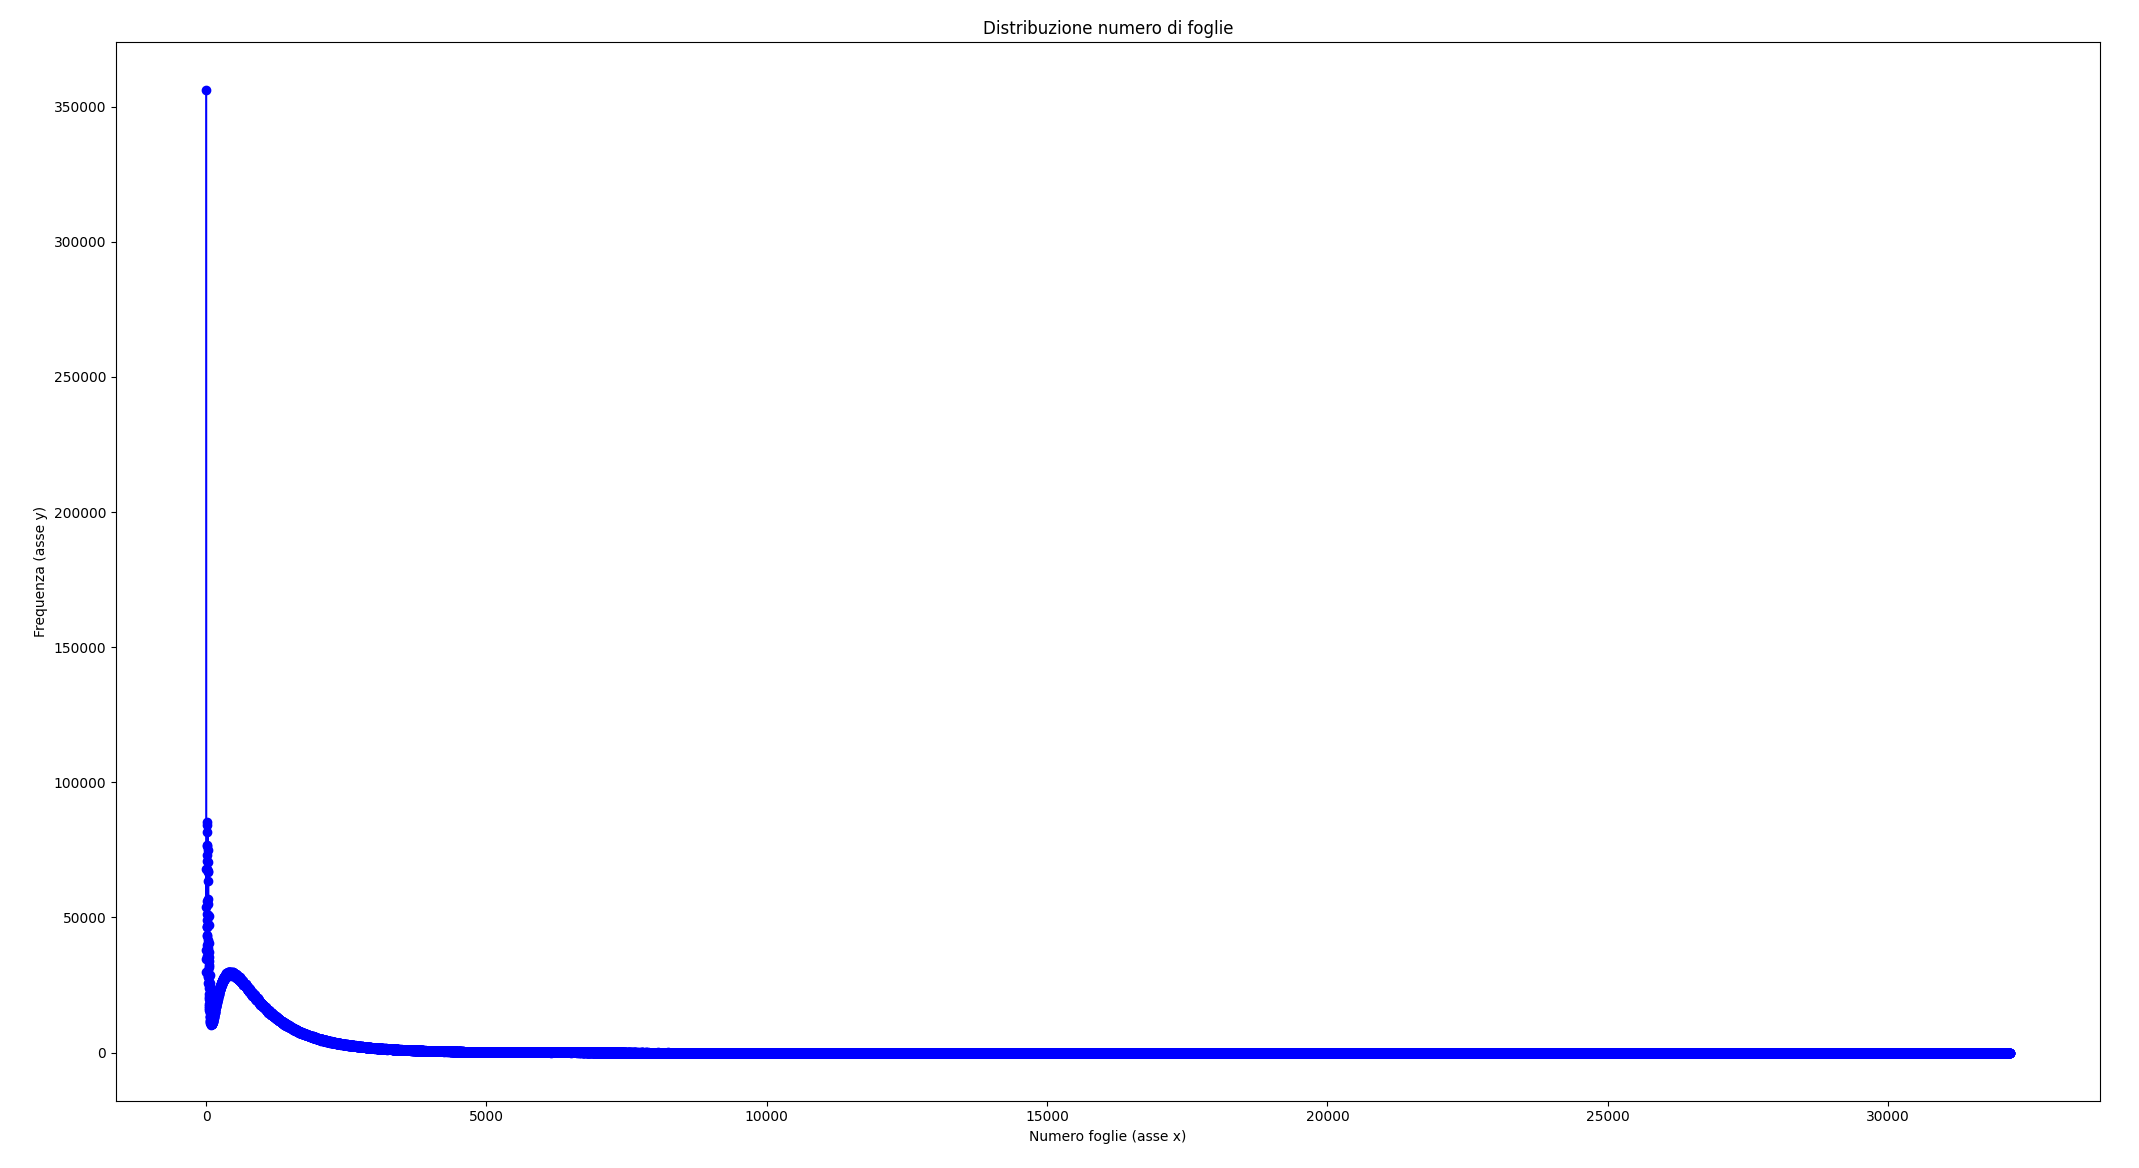
\includegraphics[width=1\textwidth]{imgs/grafico_base.png} 
    \caption{Grafico generale}
    \label{fig:etichetta}
\end{figure}

Si nota subito il picco sul valore 0, indicando che ci sono 356.142 partite con una sola foglia, corrispondenti approssimativamente a un 9\% del totale delle partite testate.


\begin{figure}[h!]
    \centering
    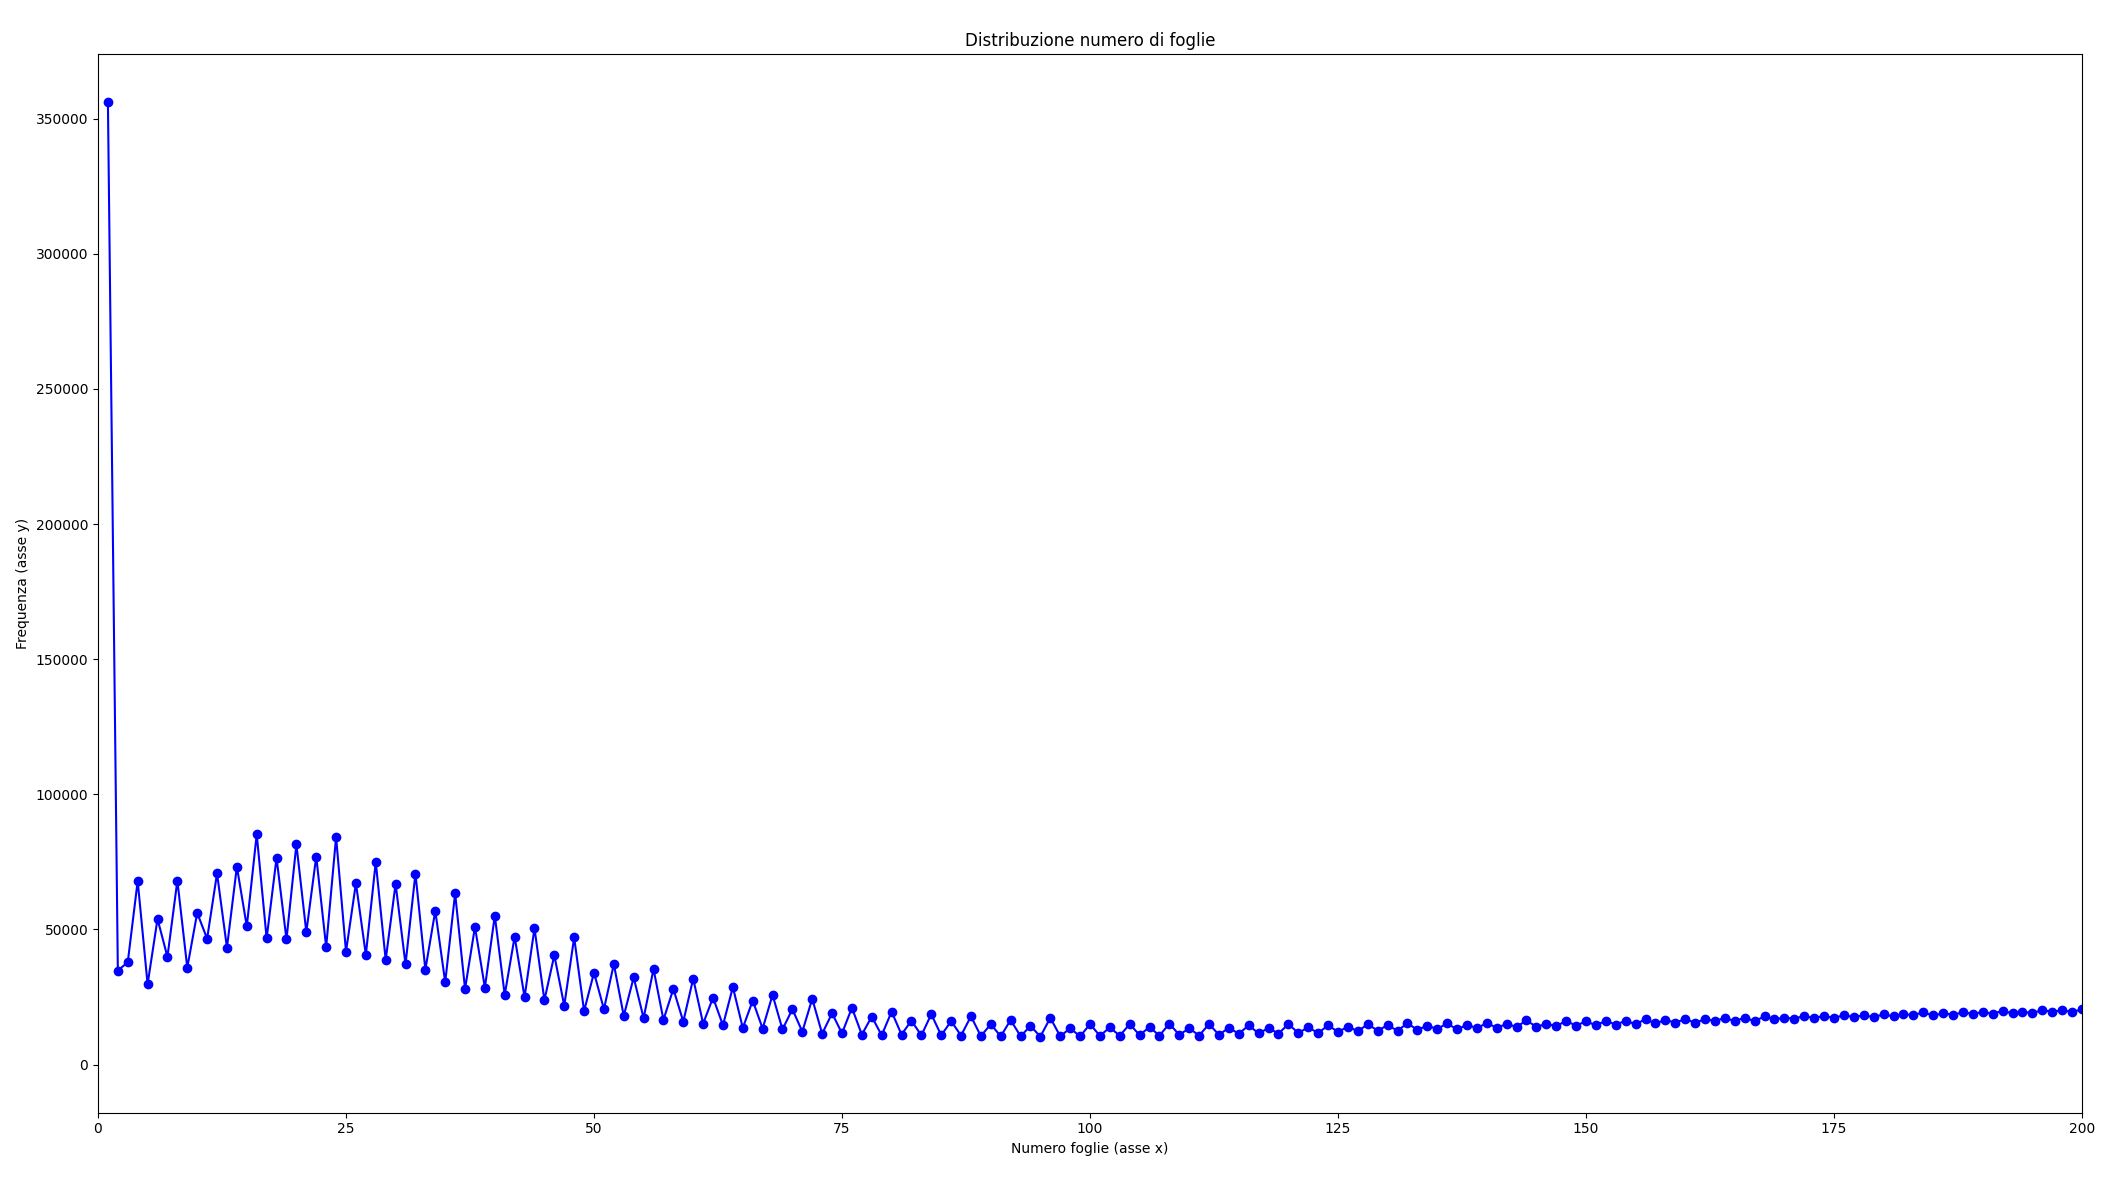
\includegraphics[width=1\textwidth]{imgs/grafico_0_200.png} 
    \caption{Ingrandimento dominio 0-200}
    \label{fig:etichetta}
\end{figure}

Curiosa l'alternanza dei valori, probabilmente solo una coincidenza che non porta a nulla di significativo.

\begin{figure}[h!]
    \centering
    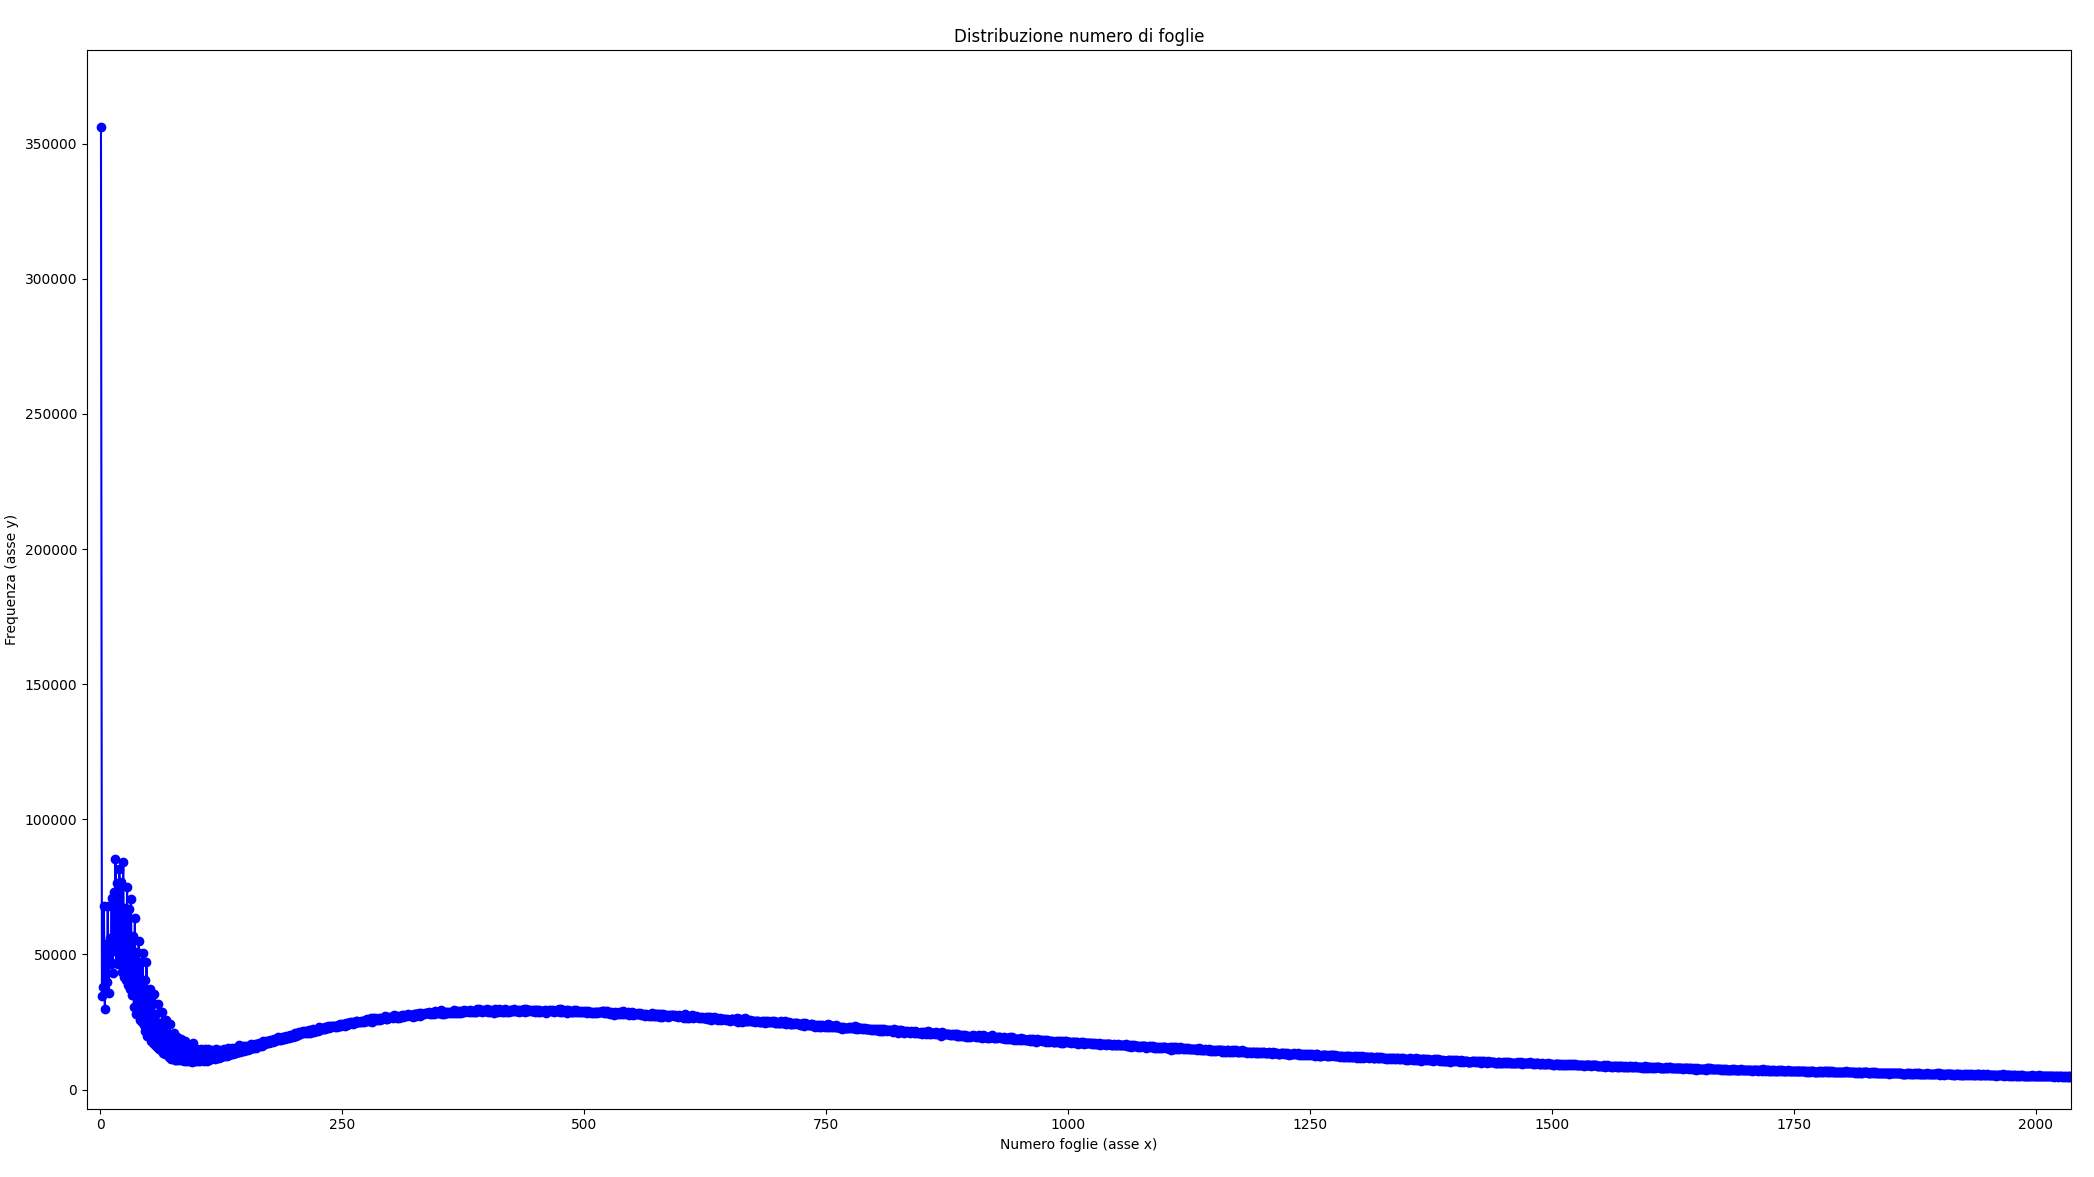
\includegraphics[width=1\textwidth]{imgs/grafico_0_2000.png} 
    \caption{Ingrandimento dominio 0-2000}
    \label{fig:etichetta}
\end{figure}

\begin{figure}[h!]
    \centering
    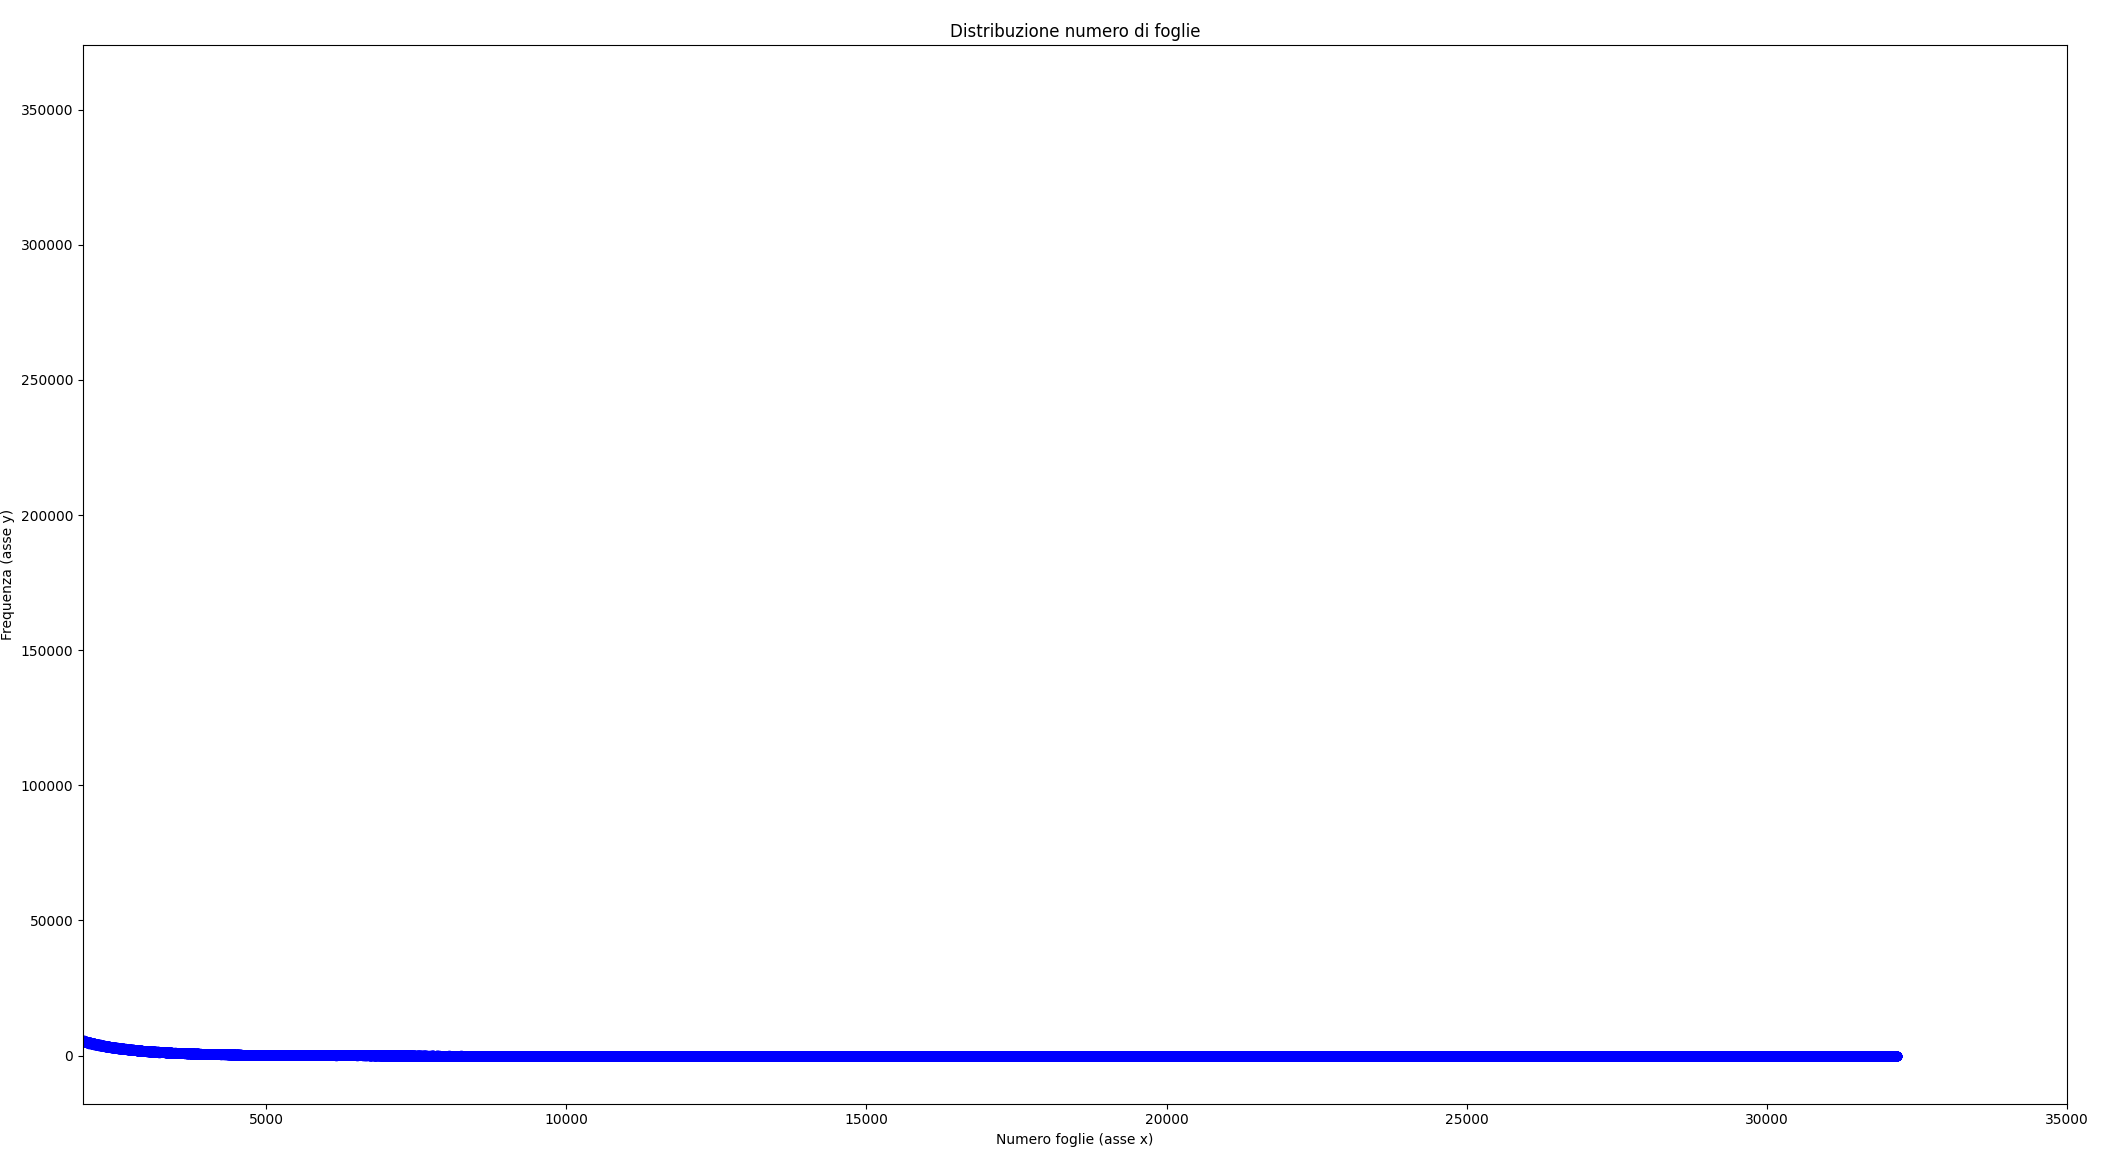
\includegraphics[width=1\textwidth]{imgs/grafico_2000_35000.png} 
    \caption{Ingrandimento dominio 2000-35000}
    \label{fig:etichetta}
\end{figure}




\chapter{Conclusioni}

Una conclusione notevole è aver verificato che i set del tipo \(x|0\ ...\ x|6\) offrono certezza di vittoria se giocati in modo corretto.

\chapter{Altro (da sistemare)}





\appendix
\chapter{Codice sorgente}
% Includi eventuali porzioni di codice

\bibliographystyle{plain} % Stile della bibliografia
\bibliography{bibliografia} % File .bib con riferimenti

\end{document}
